\documentclass[12pt,aspectratio=169]{beamer}

\usepackage{amsmath,amssymb}
\usepackage{graphicx}
\usepackage{caption}
\usepackage[english]{babel}
\usepackage{ragged2e}
\usepackage{blindtext}
\usepackage{framed}
\usepackage{cancel}
\usepackage{lipsum}
\usepackage{tikz}
\usepackage{textcomp}
\usepackage{silence}
\usepackage{catchfile}

%\usepackage{multimedia} % for movies
%\usepackage[draft]{animate}    % for animations
\usepackage{animate}    % for animations
%\renewcommand{\animategraphics}[5][]{\includegraphics[width=0.5\linewidth]{#3#4}}\renewcommand{\animategraphics}[5][]{\ErrorsOff[xkeyval]\ErrorsOff[keyval]\includegraphics[#1]{#3#4}}


% Bibliography
% \usepackage[style=alphabetic,sorting=nyt,sortcites=true,maxbibnames=9,autopunct=true,babel=hyphen,hyperref=true,abbreviate=false,backref=true,backend=biber]{biblatex}



\usepackage[backend=bibtex]{biblatex}
\addbibresource{literature.bib}

\usepackage{mathtools}
\mathtoolsset{showonlyrefs}



\renewcommand{\CancelColor}{\color{red}} %change cancel color to red

\makeatletter
\let\my@cancelto\cancelto %copy over the original cancelto command
\newcommand<>{\cancelto}[2]{\alt#3{\my@cancelto{#1}{#2}}{\mathrlap{#2}\phantom{\my@cancelto{#1}{#2}}}}
% redefine the cancelto command, using \phantom to assure that the
% result doesn't wiggle up and down with and without the arrow
\makeatother



\newenvironment{wide}[1]{\begin{columns}\column{\dimexpr\paperwidth-#1}}{\end{columns}}

\newenvironment{wide2}[2][1ex]{\begin{columns}\column{\dimexpr\paperwidth-#2}
\begin{minipage}[t][\textheight-#1]{\textwidth}
}{\end{minipage}\end{columns}}


% \definecolor{beamer@blendedblue}{rgb}{0.07,0.20,0.47}
% \setbeamercolor{structure}{fg=beamer@blendedblue}

\definecolor{bblue}{rgb}{0.2,0.2,0.7} % beamer blue
\definecolor{darkred}{rgb}{0.8,0,0}
\definecolor{litered}{rgb}{0.2,1,1}
\definecolor{Darkred}{rgb}{0.7,0,0}
\definecolor{liteyellow}{rgb}{1,1,0.7}
\definecolor{litegreen}{rgb}{0.8,1,0.8}
\definecolor{darkgreen}{rgb}{0,0.5,0}
\definecolor{litelitegray}{rgb}{0.8,0.8,0.8}
\definecolor{litegray}{rgb}{0.6,0.6,0.6}
\definecolor{purple}{rgb}{0.58,0,0.58}
\definecolor{darkmag}{rgb}{0.5,0.0,0.5}
\definecolor{darkorange}{rgb}{0.68,0.28,0.04}
\definecolor{darkbrown}{rgb}{0.55,0.35,0.15}





\newcommand<>{\altfixed}[2]{\alt#3{#1}{\mathrlap{#2}\phantom{#1}}}
\newcommand<>{\altfixedother}[2]{\alt#3{\mathrlap{#1}\phantom{#2}}{#2}}



\renewcommand<>{\mathcolorboxalt}[2]{
	\altfixed#3{{ \setlength{\fboxsep}{0pt} \colorbox{#1}{$\displaystyle #2$}}}{#2}
}




\renewcommand<>\hlbox[2]{%
  \alt#3{\colorbox{#1}{#2}}%
  {\makebox[\dimexpr\width+2\fboxsep]{#2}\vphantom{\colorbox{#1}{#2}}}%
}
\newcommand<>{\mathhlbox}[2]{%
	\alt#3{\colorbox{#1}{$\displaystyle #2$}}%
	{\makebox[\dimexpr\width+2\fboxsep]{$\displaystyle #2$}\vphantom{\colorbox{#1}{$\displaystyle #2$}}}%
}
\newcommand<>{\mathhlboxRGB}[2]{%
	\alt#3{\colorbox[RGB]{#1}{$\displaystyle #2$}}%
	{\makebox[\dimexpr\width+2\fboxsep]{$\displaystyle #2$}\vphantom{\colorbox[RGB]{#1}{$\displaystyle #2$}}}%
}
\newcommand<>{\hlboxRGB}[2]{%
	\alt#3{\colorbox[RGB]{#1}{#2}}%
	{\makebox[\dimexpr\width+2\fboxsep]{#2}\vphantom{\colorbox[RGB]{#1}{#2}}}%
}

\newcommand<>{\mathcolorbox}[2]{
	\alt#3{\colorbox{#1}{$\displaystyle #2$}}{\colorbox{white}{$\displaystyle #2$}}%
}
\newcommand<>{\mathcolorboxRGB}[2]{
	\alt#3{\colorbox[RGB]{#1}{$\displaystyle #2$}}{\colorbox{white}{$\displaystyle #2$}}%
}

\newcommand<>{\mathaltcolorbox}[3]{% color, expr1, expr2 
	\altfixed#4{\colorbox{#1}{$\displaystyle #2$}}{\colorbox{white}{$\displaystyle #3$}}%
}

% define backslash symbol $/$
\newcommand{\bsh}[0]{\textbackslash}




% hide navigation symbols
\setbeamertemplate{navigation symbols}{}
\addtobeamertemplate{navigation symbols}{}{%
	\usebeamerfont{footline}%
	\usebeamercolor[fg]{footline}%
	\hspace{1em}%
	\insertframenumber/\inserttotalframenumber
}

% make boxes rounded
\setbeamertemplate{blocks}[rounded][shadow=false]



% footnote without number
\addtobeamertemplate{footnote}{\hskip -2em}{}
\newcommand{\footnotetextrelaxed}[1]{{\let\thefootnote\relax\footnotetext{#1}}}


\usepackage{catchfile}


% \usepackage{catchfile}
% make animate work in Texpad compiler
\CatchFileDef{\CompilationMode}{mode.txt}{}
\ifthenelse{\equal{\CompilationMode}{make }}{}{
    \renewcommand{\animategraphics}[5][]{\ErrorsOff[xkeyval]\ErrorsOff[keyval]\includegraphics[#1]{#3#4}}
    }


% ============================================================
% definitions.tex — macros for manuscript.tex
%
% Carried over from the top-level derivation log (../definitions.tex),
% trimmed of nothing, plus a small block of new macros at the end for
% symbols introduced in the Extrusion/Nucleation section (dean.tex
% "Extrusion rate": Virtual work, The nucleation threshold, Layering
% probability) that did not exist when the derivation-log definitions
% file was written. Keep the two files in sync by hand — there is no
% automated check.
% ============================================================

\newcommand{\la}{\left\langle}
\newcommand{\ra}{\right\rangle}
\newcommand{\bs}{\boldsymbol}
\newcommand{\E}{\mathbf{E}}
\newcommand{\Var}{\text{Var}}
\renewcommand{\d}{\mathrm{d}}
\renewcommand{\u}{\bs{u}}
\newcommand{\q}{\bs{q}}
\newcommand{\Q}{\mathbf{Q}}
\newcommand{\R}{\mathbb{R}}
\newcommand{\n}{\bs{n}}
\newcommand{\e}{\bs{e}}
\newcommand{\T}[0]{\mathrm{T}}
\newcommand{\pd}[2]{\frac{\partial #1}{\partial #2}}
\newcommand{\tpd}[2]{\tfrac{\partial #1}{\partial #2}}


\newcommand{\ab}{{\alpha\beta}}
\newcommand{\mn}{{\mu\nu}}
\newcommand{\abmn}{{\alpha\beta\mu\nu}}

\newcommand{\eye}{\bs{\mathrm{I}}}
\renewcommand{\v}{\mathbf{v}}
\newcommand{\x}{\mathbf{x}}
\newcommand{\f}{\mathbf{f}}
\newcommand{\s}{\mathbf{s}}
\newcommand{\g}{\mathbf{g}}
\newcommand{\G}{\mathbf{G}}
\renewcommand{\H}{\mathbf{H}}
\newcommand{\Ha}{\mathbf{H}_\text{a}}
\newcommand{\F}{\mathbf{F}}
\newcommand{\I}{\mathbf{I}}
\newcommand{\J}{\mathbf{J}}
\newcommand{\bnabla}{\boldsymbol{\nabla}}
\newcommand{\A}{\mathbf{A}}
\newcommand{\B}{\mathbf{B}}
\newcommand{\U}{\mathbf{U}}
\newcommand{\bxi}{\mathbf{\xi}}
\newcommand{\p}{\mathbf{p}}
\newcommand{\W}{\mathbf{W}}
\newcommand{\bT}{\mathbf{T}}
\newcommand{\nh}{\hat{\bs{n}}}
\newcommand{\bdelta}{\bs\delta}
\newcommand{\bsigma}{\bs\sigma}
\newcommand{\bEta}{\bs\eta}
\newcommand{\fa}{\bs{f}_\text{a}}
\renewcommand{\ss}{\mathrm{ss}}

\newcommand{\ee}{\mathrm{e}}
\newcommand{\ii}{\mathrm{i}}

\renewcommand{\k}{\bs{k}}
\renewcommand{\r}{\mathbf{r}}

\newcommand{\TT}{{\rm T}}
\newcommand{\Tr}{{\rm T}}


\newcommand{\lM}{l_{\rm M}}
\newcommand{\lm}{l_{\rm m}}

\newcommand{\elln}{\ell_{\rm n}}
\newcommand{\ellc}{\ell_{\rm c}}
\newcommand{\elld}{\ell_{\rm d}}

\newcommand{\calN}{\mathcal{N}}
\newcommand{\calF}{\mathcal{F}}
\newcommand{\calG}{\mathcal{G}}
\newcommand{\calK}{\mathcal{K}}
\newcommand{\calP}{\mathcal{P}}
\newcommand{\rmR}{\mathrm{R}}

\providecommand{\Fpair}{\calF_{\mathrm{pair}}}
\providecommand{\Fent}{\calF_{\mathrm{ent}}}
\providecommand{\Tr}{\operatorname{tr}}
\newcommand{\frev}{f_{\rm rev}}
\newcommand{\xir}{\xi_{\rm r}}
\newcommand{\ecrit}{\varepsilon_{\rm c}}
\newcommand{\sigmarho}{\sigma_\rho^2}
\newcommand{\kB}{k_\mathrm{B}}
% Correction / open-question annotations (visible in the compiled PDF —
% useful while this is still a skeleton; strip before submission)
\newcommand{\corr}[1]{\textcolor{red}{\textbf{[CORR:}\ #1\textbf{]}}}
\newcommand{\corrm}[1]{{\color{red}#1}}
\newcommand{\todo}[1]{\textcolor{purple}{\textbf{[TODO:}\ #1\textbf{]}}}

\renewcommand{\div}{\text{div}}

\newcommand{\pade}{\text{Pad\'{e}}}
\newcommand{\cell}{\text{cell}}
\newcommand{\crit}{\text{crit}}

\newcommand{\Pa}{\text{Pa}}
\newcommand{\kPa}{\text{kPa}}

\newcommand{\minute}{\text{min}}
\newcommand{\micron}{\upmu\mathrm{m}}
\newcommand{\tcdot}{\!\cdot\!}

\newcommand{\ash}[1]{\textcolor{blue}{\textbf{[ash:}\ #1\textbf{]}}}

% ------------------------------------------------------------
% New in manuscript.tex: symbols from dean.tex's "Extrusion rate"
% section (Virtual work / The nucleation threshold / Layering
% probability), which post-date the derivation-log definitions.tex.
% ------------------------------------------------------------

\newcommand{\gammaw}{\gamma_{\rm w}}           % water/interfacial surface tension (NOT the nematic relaxation rate \gamma, NOT gamma_0 = B/xi_0 — three distinct gammas in this project, see canonical-model-parameters memory)
\newcommand{\Wc}{W_{\rm c}}                    % cell-cell adhesion energy
\newcommand{\Ws}{W_{\rm s}}                    % cell-substrate adhesion energy
\newcommand{\Acell}{A_{\rm cell}}              % single-cell area
\newcommand{\pcrit}{p_{\rm crit}}              % critical pressure, boxed result eq:pcrit
\newcommand{\nuzero}{\nu_0}                    % peak variance modulation, sec-layering-probability
\newcommand{\ellA}{\ell_A}                     % nucleus smoothing scale (superseded alternative — see FRIDGE/fluctuation_mechanism.tex; kept only in case it resurfaces)


% prompt, address all the prompts in the text
\newcommand{\prompt}[1]{\textcolor{blue!90!black}{[ #1 ]}}
\newcommand{\unclear}[1]{{\color{blue}[\textit{unclear}} #1{\color{blue}]}}



\newcommand{\comment}[1]{}




%%%%%%%%%%%%%%%%%%%%%%%%%%%%%%%%%%%%%%%%%%
%%%%%%%%%%%%%%%%%%%%%%%%%%%%%%%%%%%%%%%%%%
%%%%%%%%%%%%%%%%%%%%%%%%%%%%%%%%%%%%%%%%%%
%Information to be included in the title page:
%\title{Exploring the Mechanism of Fruiting Body Formation in Myxo Colonies}
\title{From Polarity Fluctuations to Fruiting Bodies}

%\subtitle{(Myxococcus xanthus)\\\vspace{0.6cm}2024 Circle Meeting}
\author{Ashot Matevosyan\\
{\small supervisor: Ricard Alert}}
\institute{Max Planck Institute for the Physics of Complex Systems}
% Max Planck Institute for the Physics of Complex Systems
\date{\today}

%\logo{
\includegraphics[height=1cm]{media/pkslogo}}
\titlegraphic{\vspace{-1.7cm}\hspace{-0.7cm}
\includegraphics[height=1.5cm]{media/pkslogo}\hfill ~}


\begin{document}



% make animate work in Texpad compiler
%\CatchFileDef{\CompilationMode}{mode.txt}{}
%\ifthenelse{\equal{\CompilationMode}{make }}{}{
%    \renewcommand{\animategraphics}[5][]{\ErrorsOff[xkeyval]\ErrorsOff[keyval]\includegraphics[#1]{#3#4}}
%    }



\comment{
\setbeamertemplate{background}{
\tikz[overlay, remember picture,
    every path/.style={opacity=0.1, black,very thick},
    shift=(current page.south west),
    x=(current page.south east), y=(current page.north west),
  ]{
  \draw[step=1cm, thick] (0,0) grid (1,1);
  \draw (1/3,0) -- (1/3,1);
  \draw (2/3,0) -- (2/3,1);
  \draw (0,1/3) -- (1,1/3);
  \draw (0,2/3) -- (1,2/3);
  \draw[opacity=0.8, black,ultra thick] (0,0) -- (1,0);
  }
\tikz[overlay, remember picture,
    shift=(current page.center)
  ]{\filldraw[black,opacity=0.2] (0,0) circle (2pt);}
}
}


\frame{\titlepage}





{
\setbeamertemplate{background canvas}{
\begin{tikzpicture}[remember picture, overlay, shift={(current page.center)}]       
\node (fig1) at (0,0){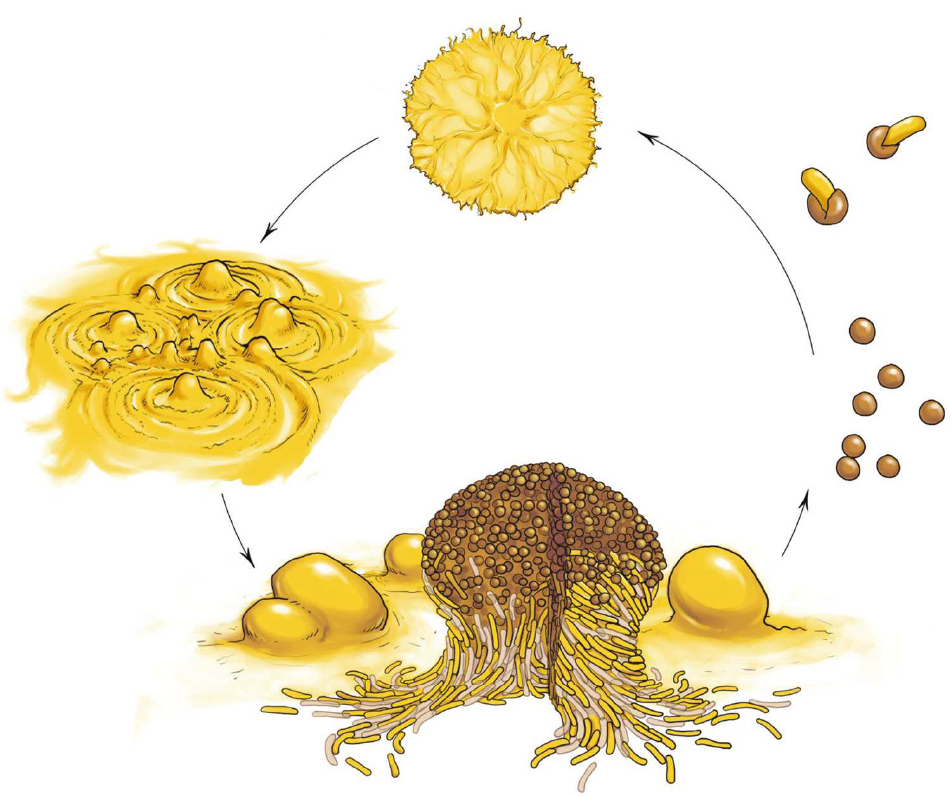
\includegraphics[height=0.85\paperheight]{media/myxo-life}};   
\end{tikzpicture}
}
\begin{frame}{The life cycle of Myxo}

\tikz[overlay,remember picture,
shift=(current page.center),
every node/.style={fill=none,text=black}]{
\node at (-2,3) {Swarming};
\node at (-6,0.8){Aggregation};
\node at (-5,-2.8){Fruiting bodies};
\node at (5.3,-1.2){Sporulation};
\node at (5.1,1.9){Germination};
}%
\pause
\tikz[overlay,remember picture,
shift=(current page.center),
every node/.style={fill=none,text=black}]{
\draw[->,line width=6,red] (-1,2.5) .. controls +(-0.6,-0.4) .. (-2.1,1.5);
}%


\footnotetextrelaxed{\fullcite{munoz2016myxobacteria}}
\end{frame}
}


\begin{frame}[t]
\begin{wide}{10pt}

\begin{minipage}{0.35\linewidth}
\vspace{1cm}
\centering
\includegraphics<1>[width=0.95\linewidth]{media/fruitingbody/img000}%
\only<2->{%
\animategraphics[autoplay,loop,width=0.95\linewidth,timeline=media/fruitingbody/timeline.txt]{15}{media/fruitingbody/img}{000}{152}}
\end{minipage}%
\hfill
\begin{minipage}{0.64\linewidth}
\alt<3->{
\animategraphics[autoplay,loop,width=\linewidth]{30}{media/colony/img}{00}{95} 
}{\phantom{\animategraphics[draft,autoplay,loop,width=\linewidth]{30}{media/colony/img}{00}{95}}
}
\end{minipage}
\end{wide}
\footnotetextrelaxed{(left) \fullcite{curtis2007spatial}}
\footnotetextrelaxed{\onslide<3->{(right)\fullcite{copenhagen}}}
\vspace{-2cm}
\end{frame}




\begin{frame}{Probability of Layer Formation}
\vspace{-1cm}
\begin{wide}{10pt}
\begin{minipage}{0.6\linewidth}
\vspace{1cm}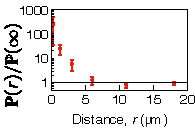
\includegraphics[width=0.8\linewidth]{media/prob_experiment}

\vspace{-3ex}\hfill
\alt<2>{\includegraphics[page=2,width=2cm,trim={0 0 3cm 0},clip]{media/defect-ilustration.pdf}}
{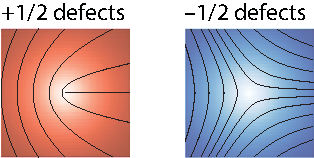
\includegraphics[page=1,width=2cm,trim={0 0 3cm 0},clip]{media/defect-ilustration.pdf}}

\end{minipage}%
\hfill%
\begin{minipage}{0.3\linewidth}
\animategraphics[autoplay,loop,width=0.8\linewidth]{15}{media/defect1/defect1_}{00}{68}

\vspace{1ex}
\animategraphics[autoplay,loop,width=0.8\linewidth]{15}{media/defect2/defect2_}{00}{68}
\end{minipage}

\end{wide}
\footnotetextrelaxed{\fullcite{copenhagen}}
\end{frame}




\comment{
\begin{frame}[t]{Compressibility}
%\centering
\begin{wide}{30pt}
\vspace{-0.2cm}

\hspace{2.8cm}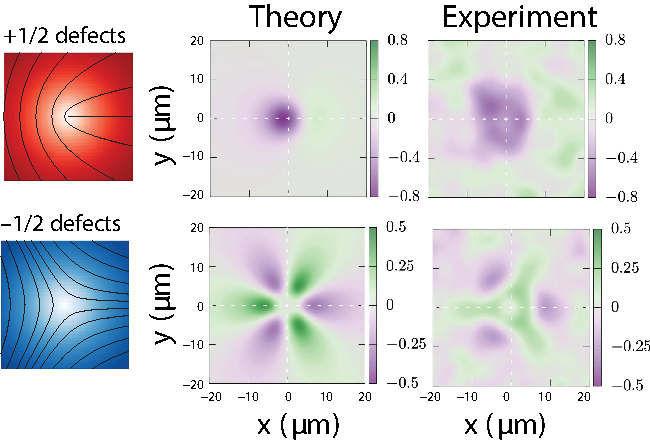
\includegraphics[height=0.83\paperheight-4cm,trim={0cm 4cm 0cm 0cm},clip]{media/divergence_of_v}
\vspace{0.5cm}

\center{\large \begin{minipage}{0.8\linewidth}
System is 
\begin{itemize}
    \item Incompressible \textbf{before} layer formation
    \item Compressible \textbf{during} layer formation
\end{itemize}
\end{minipage}}
\end{wide}
\end{frame}
}


\begin{frame}{\large Large fluctuations \\ in the system}
    \vspace{-9ex}
\begin{wide}{5pt}
    \hfill 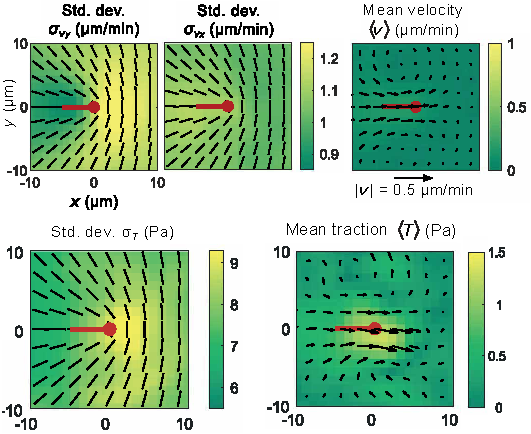
\includegraphics[width=0.65\linewidth]{media/experiment-slide}

\end{wide}
% \vspace{-1ex}

{\footnotesize \fullcite{preprint}}
\end{frame}





\begin{frame}[t]{\large Traction force measurement}
\footnotetextrelaxed{\fullcite{preprint}} 

\includegraphics<1>[page=4,width=\linewidth]{media/layer_formation}%
\includegraphics<2>[page=5,width=\linewidth]{media/layer_formation}%
\includegraphics<3-4>[page=6,width=\linewidth]{media/layer_formation}%
\vspace{-2.3ex}
\center{
\onslide<2->{\color[RGB]{180,0,0} Fluorescent beads}%\hspace{1cm}
\hfill
\onslide<3->{\color[RGB]{0,150,0} Traction Force}
}

\onslide<4->{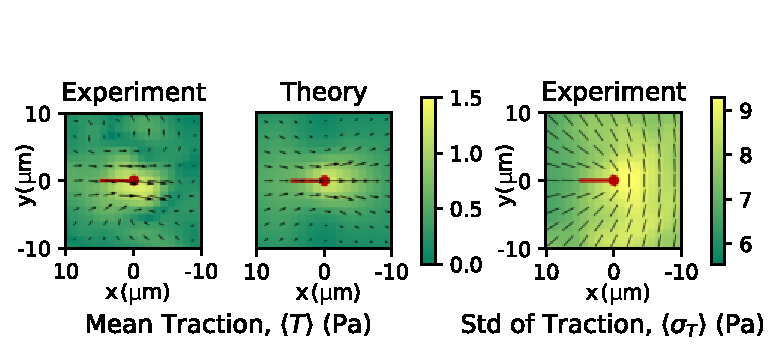
\includegraphics[width=0.9\linewidth,trim={0 0 0 1cm},clip]{media/traction}}
\vspace{-10ex}
   
\end{frame}




\begin{frame}[t]{\large Polarity measurement}
\vspace{-3ex}
\begin{wide}{10pt}
\centering
% \hfill
\begin{minipage}{0.3\linewidth}
    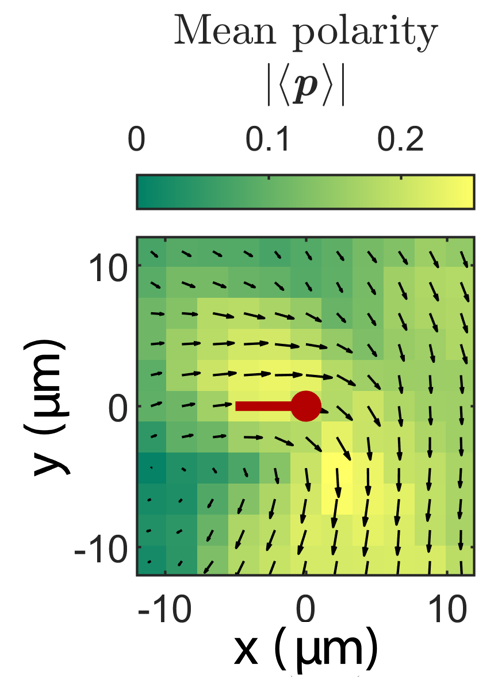
\includegraphics[width=0.9\linewidth]{media/polarity-mean}
\end{minipage}%
\begin{minipage}{0.3\linewidth}
    {\footnotesize ~~~~~~Std. dev. of polarity}

    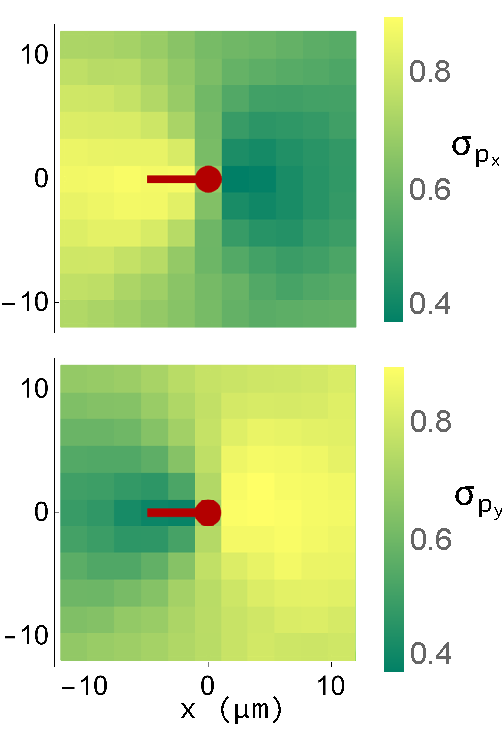
\includegraphics[height=0.85\paperheight]{media/experiment-p-fluctuations}
\end{minipage}~~%
\begin{minipage}{0.3\linewidth}
    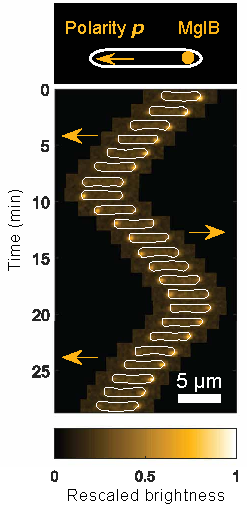
\includegraphics[height=0.9\paperheight]{media/polarity measurement}
\end{minipage}%
\end{wide}
\vspace{-10ex}
\footnotetextrelaxed{\fullcite{preprint}} 
\end{frame}




\begin{frame}{Outline}
\onslide<+->
\begin{wide}{10pt}
\begin{minipage}[t]{0.5\linewidth}
    
    \vspace{1cm}
    \begin{itemize}
    \setlength\itemsep{3ex}

    \item average fields are not strong enough for layer formation
    \item Fluctuations in the system are large
    \item \textbf{  \color{bblue}Hypothesis:} fluctuations drive \\ \hfill layer formation.~~~~
\end{itemize}
\end{minipage}% 
\hfill\onslide<+->
\begin{minipage}[t]{0.5\linewidth}
    
{\centering

\vspace{1cm}Polarity fluctuations     

\vspace{0.5cm}
$\big\downarrow$

\vspace{0.5cm}
Pressure fluctuations

\vspace{0.5cm}
$\big\downarrow$

\vspace{0.5cm}
{\color<+->{darkgreen} 
\textbf<.->{Nucleation Theory}}

\vspace{1cm}
}

\end{minipage}
\end{wide}
\end{frame}









\begin{frame}[t]{Energetics of Layer Formation}\onslide<+->
\includegraphics<1>[page=1,width=\linewidth]{media/layer_formation}%
\includegraphics<2-4>[page=2,width=\linewidth]{media/layer_formation}%
\only<5>{\animategraphics[autoplay,width=\linewidth]{10}{media/layer_formation_anim}{0}{8}}%
\includegraphics<6->[page=9,width=\linewidth]{media/layer_formation_anim}%
\onslide<+->
\onslide<+->
\vspace{1ex} 

\begin{wide}{10pt}
\begin{minipage}{0.5\linewidth}
\begin{itemize}
    \item detach from substrate: $\color{Darkred} W_{cs} A$,
    \item detach from neighbours: $\color{Darkred} W_{cc} h\;\ell$,
    \item surface tension of water: $\color{Darkred} \gamma_w h\;\ell$,
\end{itemize}
\end{minipage}%
\begin{minipage}{0.5\linewidth}
%\pause\pause
\temporal<.-.(2)>{}{\centering $\ell$ is perimeter}{
\begin{itemize}
    \item adhere to bottom cells: $\color{bblue}-W_{cc} A$,
    \item release pressure: $\color{bblue}-E_p$. 
\end{itemize}
}
\end{minipage}

\only<.(1)-.(3)>{\center{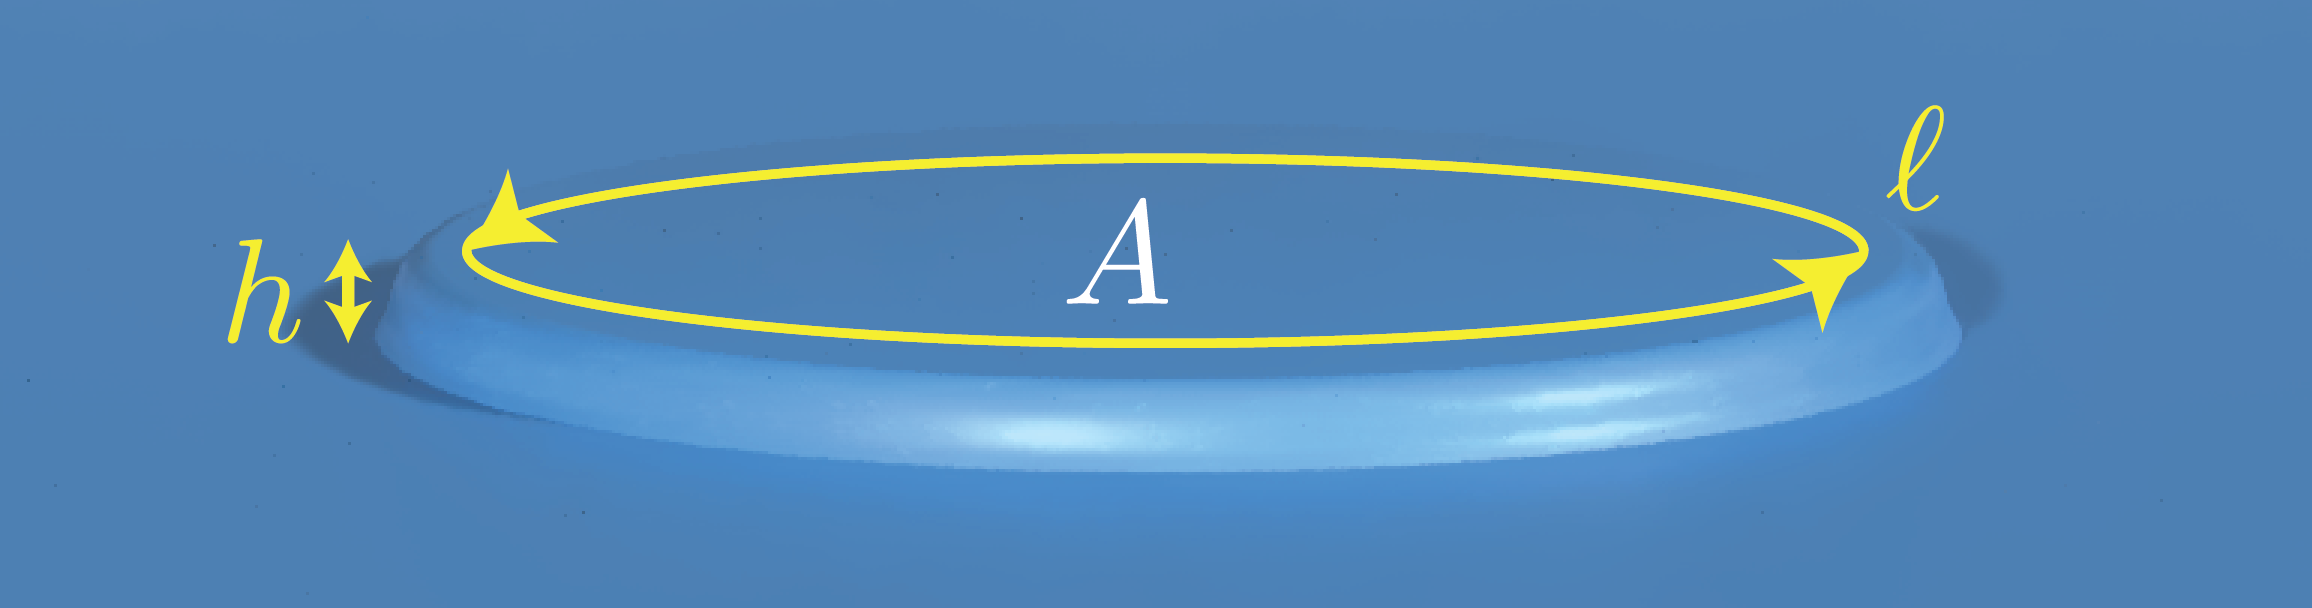
\includegraphics[width=0.8\textwidth]{media/layer_formation_3d_png}}}
\onslide<+(2)->\vspace{0ex}
\vspace{1ex}
\onslide<+->\onslide<+->\onslide<+->

\begin{equation}
    \Delta E={\color{Darkred}W_{cs} A+W_{cc} h\;\ell+\gamma_w h\;\ell}{\color{bblue} -W_{cc} A - E_p}
\end{equation}
\onslide<+->
\vspace{-0.8cm}
\begin{align}
    \onslide<+->{A=\pi (\ell/2)^2 \approx \ell^2} \qquad\qquad E_p(A,\,p) \approx p\;hA 
\end{align}
\onslide<+->
\vspace{-1em}
\begin{equation}
\Delta E({\color{darkgreen} A},\,p)=(W_{cs}-W_{cc}) {\color{darkgreen} A} + (W_c+\gamma_w) h\;\sqrt{{\color{darkgreen} A}}- E_p({\color{darkgreen} A},\,p)
\end{equation}
\end{wide}
\end{frame}








\begin{frame}{Energy Barrier} 
\vspace{-0.5cm}
\begin{equation}
{\color{bblue}\Delta E(A,\,p)}=(W_{cs}-W_{cc}) A + (W_c+\gamma_w) h\;\sqrt{A}- \overbrace{ p\,hA}^{{\color{darkgreen}E_p(A,\,p)}}
\end{equation}
\bigskip

\hfill
\includegraphics<1>[height=0.8\paperheight,trim={1.5cm 0cm 0cm 1cm},clip]{media/barier/frames/frame4001}%
\includegraphics<2>[height=0.8\paperheight,trim={1.5cm 0cm 0cm 1cm},clip]{media/barier/frames/frame4002}%
\includegraphics<3->[height=0.8\paperheight,trim={1.5cm 0cm 0cm 1cm},clip]{media/barier/frames/frame4003}%
\hspace{1cm}

\end{frame}

\begin{frame}{Barrier Fluctuations}
\hfill
\animategraphics[autoplay,loop,height=0.85\paperheight]{80}{media/barier/frames/frame}{000}{079}
\hspace{1cm}
    
\end{frame}






\begin{frame} 
\begin{wide}{10pt}
\vspace{0.5ex} 
\onslide<+->
\begin{minipage}[t]{0.47\linewidth}
\centerline{ {\color<2->{litelitegray}Average} pressure around $+\tfrac{1}{2}$ defect}
\includegraphics<1>[width=1.\linewidth]{media/pressure-on-defect}%  
\only<2->{\animategraphics[autoplay,loop,width=1\linewidth]{5}{media/pressure-frames/frame}{1}{5}}     
\end{minipage}%
\begin{minipage}[t]{0.5\linewidth}
\onslide<+->
$$p(\r) =\la p(\r) \ra + {\color{purple} \delta p(\r)} \onslide<.(1)->{\color{darkred} \quad> p_c}$$
$${\color{purple} \delta p(\r)} \sim \mathhlbox<5->{litegreen}{\mathcal{N}(0,\sigma_p(\r)^2)}$$
\end{minipage}
%\vspace{-7.8ex}
\vspace{-5.8ex}
\onslide<+->\onslide<+->

\hfill\onslide<.(1)->{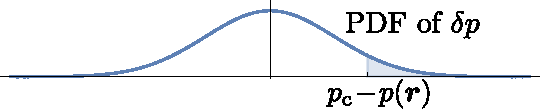
\includegraphics[width=0.65\linewidth]{media/normal_tail}}
\vspace{-0.2cm}
$$\mathbb{P}\left(\text{New layer} \atop\text{at point }{\r}\right)=\mathbb{P}\Big({\color{purple} \delta p} > {\color{darkred} p_c}-\la p(\r) \ra\!\Big)
\onslide<+->
\onslide<+->
=1-\text{Erf}\left(\frac{{\color{darkred} p_c}-\la p(\r)\ra}{\sigma_p(\r)}\right)$$
\vspace{-2ex}
%\onslide<+->
%$$1-\text{Erf}(x)\approx \tfrac{1}{\sqrt{\pi}}\;\ee^{-x^2}/x$$
\end{wide}

\end{frame}





\begin{frame}[t] 
\begin{minipage}{0.6\linewidth}

\end{minipage}%
\hfill%
\begin{minipage}{0.4\linewidth}
{\Large \color{bblue} ~~Outline}

{\centering

\vspace{1cm}

\alt<2->{{{\color{bblue}Microscopic model}}}{{\color{darkred}Polarity fluctuations}}
   

\vspace{0.5cm}
$\big\downarrow$

\vspace{0.5cm}
{\color{darkred}Pressure fluctuations}

\vspace{0.5cm}
$\big\downarrow$

\vspace{0.5cm}
{\color{darkgreen}Nucleation Theory {\Large \checkmark}}

\vspace{1cm}
}
\end{minipage}%
\end{frame}


% ---------------------------------------------------------------------------
% colour code: interactions / self-propulsion & reversals / rotational noise;
% in the Dean frames: interactions / thermal noise / diffusion (Ito)
\newcommand{\colI}[1]{{\color{bblue}#1}}
\newcommand{\colA}[1]{{\color{darkred}#1}}
\newcommand{\colR}[1]{{\color{darkgreen}#1}}
\newcommand{\colN}[1]{{\color{darkgreen}#1}}
\newcommand{\colD}[1]{{\color{darkorange}#1}}
% focus: the piece being worked on
\newcommand{\hlf}[1]{{\setlength{\fboxsep}{1pt}\colorbox{liteyellow}{$#1$}}}
% small label under a term
\newcommand{\lab}[2]{\underbrace{#1}_{\text{\scriptsize #2}}}
% boxed reminder in the top-right corner of the frame body; first command of a [t] frame.
% Positioned relative to the text, so it needs no second run (no remember picture).
\newcommand{\reminder}[1]{%
\par\noindent\begin{tikzpicture}[overlay]
\node[anchor=north east,draw=litegray,rounded corners=2pt,fill=white,inner sep=3pt,font=\footnotesize]
    at (\linewidth,3ex) {#1};
\end{tikzpicture}\par\vspace{-\baselineskip}}
\newcommand{\deanlegend}{\hfill{\footnotesize \colI{interactions}\quad \colN{noise}\quad \colD{diffusion (It\^o)}}}
% ---------------------------------------------------------------------------


\begin{frame}{Microscopic model of reversing bacteria}
\onslide<+->
\begin{wide}{30pt}
\begin{minipage}[c]{0.4\linewidth}
    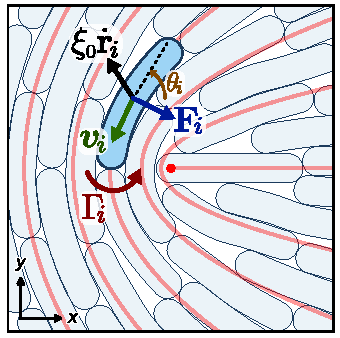
\includegraphics[width=\linewidth,page=1]{media/paper-main}
\end{minipage}%
\begin{minipage}[c]{0.6\linewidth}
    \small\setlength{\abovedisplayskip}{3pt}\setlength{\belowdisplayskip}{3pt}
    \begin{align*}
        \frac{\d\r_i}{\d t} &= \colI{\frac{\rho_0}{\xi_0}\F_i} + \colA{v_0\,\p(\theta_i)\, k_i}
        \\
        \frac{\d\theta_i}{\d t} &= \colI{\frac{\rho_0}{\xir}\Gamma_i} + \colR{\lambda_i}
        \\[1ex]
        \onslide<2->{\colA{\la k_i(t)k_j(t')\ra}} &\onslide<2->{= \delta_{ij}\,\ee^{-2\frev|t-t'|}}
        \\
        \onslide<2->{\colR{\la\lambda_i(t)\lambda_j(t')\ra}} &\onslide<2->{= 2\Lambda\,\delta_{ij}\,\delta(t-t')}
        \\[1ex]
        \onslide<3->{\colI{\F_i}} &\onslide<3->{= -\pd{}{\r}\textstyle\sum_{j} V(\r_i-\r_j,\theta_i,\theta_j)}
        \\
        \onslide<3->{\colI{\Gamma_i}} &\onslide<3->{= -\pd{}{\theta}\textstyle\sum_{j} V(\r_i-\r_j,\theta_i,\theta_j)}
    \end{align*}
    {\footnotesize
    \onslide<2->{reversals: $\colA{k_i=\pm1}$, switching at rate $\frev$}

    \onslide<4->{$V(\r-\r',\theta,\theta')=V(\r'-\r,\theta',\theta)$ $\Rightarrow$ no self force}}
\end{minipage}

\end{wide}
\vspace{2ex}
\onslide<1->
\hfill{\footnotesize \colI{interactions}\quad \colA{self-propulsion \& reversals}\quad \colR{rotational noise}}
\end{frame}


\begin{frame}[t]{Stochastic density functional theory: Dean's equation}
\small\setlength{\abovedisplayskip}{4pt}\setlength{\belowdisplayskip}{4pt}
\onslide<+->
Brownian particles, pair potential $V$:
\begin{align*}
    \frac{\d X_i}{\d t} = \lab{\colN{\eta_i(t)}}{thermal noise} - \lab{\colI{\sum_{j=1}^N \nabla V\big(X_i - X_j\big)}}{pair forces},
    \qquad
    \colN{\la \eta_i^\mu(t)\,\eta_j^\nu(t')\ra} = 2T\,\delta_{ij}\,\delta^{\mu\nu}\,\delta(t-t')
\end{align*}
\onslide<+->
Densities:
\begin{align*}
    \varrho_i(x,t) = \delta\big(X_i(t)-x\big),
    \qquad
    \varrho(x,t) = \sum_{i=1}^N \varrho_i(x,t)
\end{align*}
\onslide<+->
Test function $\hlf{f}$:
\begin{align*}
    \hlf{f}\big(X_i(t)\big) = \int\!\d x\;\varrho_i(x,t)\,\hlf{f(x)}
    \quad\onslide<+->{\Longrightarrow\quad
    \frac{\d f(X_i)}{\d t} = \int\!\d x\;\hlf{f(x)}\,\pd{\varrho_i(x,t)}{t}}
\end{align*}
\onslide<+->
\textbf{Idea:} compute $\d f(X_i)/\d t$ with It\^o, compare

\onslide<1->
\vfill
\deanlegend
\footnotetextrelaxed{\fullcite{dean1996}}
\end{frame}


\begin{frame}[t]{Dean's equation: It\^o for one particle}
\small\setlength{\abovedisplayskip}{4pt}\setlength{\belowdisplayskip}{4pt}
\reminder{$\frac{\d X_i}{\d t} = \colN{\eta_i} - \colI{\sum_{j}\nabla V(X_i - X_j)}$}
\onslide<+->
It\^o's lemma, expanded to second order in $\d X_i$:
\begin{align*}
    \d f(X_i) = \nabla f(X_i)\cdot\d X_i + \tfrac12\,\partial_\mu\partial_\nu f(X_i)\,\d X_i^\mu\,\d X_i^\nu,
    \qquad
    \d X_i^\mu\,\d X_i^\nu = 2T\delta^{\mu\nu}\d t
\end{align*}
\onslide<+->
Insert $\d X_i$:
\begin{align*}
    \frac{\d f(X_i)}{\d t}
    = \colN{\nabla f(X_i)\cdot\eta_i}
    - \colI{\nabla f(X_i)\cdot\sum_{j}\nabla V\big(X_i-X_j\big)}
    + \lab{\colD{T\,\nabla^2 f(X_i)}}{It\^o}
\end{align*}
\onslide<+->
Every term is a function $g(X_i)$; write it as $g(X_i)=\int\!\d x\;\varrho_i(x,t)\,g(x)$:
\begin{align*}
    \frac{\d f(X_i)}{\d t}
    = \int\!\d x\;\varrho_i\Big[
    \colN{\hlf{\nabla f}\cdot\eta_i}
    - \colI{\hlf{\nabla f}\cdot\sum_{j}\nabla V\big(x-X_j\big)}
    + \colD{T\,\hlf{\nabla^2 f}}
    \Big]
\end{align*}

\footnotetextrelaxed{\fullcite{dean1996}}
\end{frame}


\begin{frame}[t]{Dean's equation: one particle}
\small\setlength{\abovedisplayskip}{4pt}\setlength{\belowdisplayskip}{4pt}
\reminder{$\frac{\d X_i}{\d t} = \colN{\eta_i} - \colI{\sum_{j}\nabla V(X_i - X_j)}$}
\onslide<+->
\vspace{1ex}
From It\^o:
\begin{align*}
    \frac{\d f(X_i)}{\d t}
    = \int\!\d x\;\varrho_i\Big[
    \colN{\hlf{\nabla f}\cdot\eta_i}
    - \colI{\hlf{\nabla f}\cdot\sum_{j}\nabla V\big(x-X_j\big)}
    + \colD{T\,\hlf{\nabla^2 f}}
    \Big]
\end{align*}
\onslide<+->
Integrate by parts, derivatives move from $\hlf{f}$ onto $\varrho_i$:
\begin{align*}
    \frac{\d f(X_i)}{\d t}
    = \int\!\d x\;\hlf{f}\Big[
    \colN{-\nabla\cdot\big(\varrho_i\,\eta_i\big)}
    + \colI{\nabla\cdot\Big(\varrho_i\sum_{j}\nabla V\big(x-X_j\big)\Big)}
    + \colD{T\,\nabla^2\varrho_i}
    \Big]
\end{align*}
\onslide<+->
Compare with $\displaystyle \frac{\d f(X_i)}{\d t} = \int\!\d x\;\hlf{f}\;\partial_t\varrho_i$, $\forall f$:
\begin{align*}
    \boxed{\pd{\varrho_i(x,t)}{t}
    = \colN{-\nabla\cdot\big(\varrho_i\,\eta_i\big)}
    + \colI{\nabla\cdot\Big(\varrho_i\sum_{j}\nabla V\big(x-X_j\big)\Big)}
    + \colD{T\,\nabla^2\varrho_i}}
\end{align*}
\onslide<+->
no noise average: one realization

\footnotetextrelaxed{\fullcite{dean1996}}
\end{frame}


\begin{frame}[t]{Dean's equation: summing over particles}
\small\setlength{\abovedisplayskip}{4pt}\setlength{\belowdisplayskip}{4pt}
\onslide<+->
One particle:
\begin{align*}
    \pd{\varrho_i}{t}
    = \colN{-\nabla\cdot\big(\varrho_i\,\eta_i\big)}
    + \colI{\nabla\cdot\Big(\varrho_i\sum_{j}\nabla V\big(x-X_j\big)\Big)}
    + \colD{T\,\nabla^2\varrho_i}
\end{align*}
\onslide<+->
Sum over $i$:
~~~\onslide<2->{$\sum_i\varrho_i = \varrho$}
~~~~~~\onslide<5->{$\sum_j g(X_j) = \int\!\d y\;\varrho(y,t)\,g(y)$}
\begin{align*}
    \pd{\varrho}{t}
    = \colN{-\sum_{i}\nabla\cdot\big(\varrho_i\,\eta_i\big)}
    + \colI{\nabla\cdot\Big(
      \altfixed<-3>{\textstyle\sum_i\varrho_i}{~~~\hlf{\varrho}}\,
      \altfixedother<-5>{~~~\textstyle\sum_{j}\nabla V\big(x-X_j\big)}{\hlf{\textstyle\int\!\d y\;\varrho(y,t)\,\nabla V(x-y)}}
    \Big)}
    + \colD{T\,\nabla^2\altfixed<-2>{\textstyle\sum_i\varrho_i}{\hlf{\varrho}}}
\end{align*}

\onslide<7->
Drift closed in $\varrho$; noise is not:
\begin{align*}
    \colN{\xi(x,t)} = \colN{-\sum_{i}\nabla\cdot\big(\varrho_i\,\eta_i\big)}
\end{align*}

\footnotetextrelaxed{\fullcite{dean1996}}
\end{frame}


\begin{frame}[t]{Dean's equation: free energy}
\small\setlength{\abovedisplayskip}{4pt}\setlength{\belowdisplayskip}{4pt}
\onslide<+->
\begin{align*}
    \pd{\varrho}{t}
    = \colI{\nabla\cdot\Big(\varrho\int\!\d y\;\varrho(y,t)\,\nabla V(x-y)\Big)}
    + \colD{T\,\nabla^2\varrho}
    + \colN{\xi}
\end{align*}
\onslide<+->
\begin{align*}
    F[\varrho] = \lab{\colI{\frac12\int\!\d x\,\d y\;\varrho(x)\,V(x-y)\,\varrho(y)}}{interaction energy}
    + \lab{\colD{T\!\int\!\d x\;\varrho(x)\log\varrho(x)}}{ideal-gas entropy}
\end{align*}
\onslide<+->
\begin{align*}
    \frac{\delta F}{\delta\varrho(x)} &= \colI{\int\!\d y\;V(x-y)\,\varrho(y)} + \colD{T\big(\log\varrho(x)+1\big)},
    &&\text{\footnotesize $V(x)=V(-x)$}
    \\
    \varrho\,\nabla\frac{\delta F}{\delta\varrho} &= \colI{\varrho\!\int\!\d y\;\varrho(y)\,\nabla V(x-y)} + \colD{T\,\nabla\varrho}
\end{align*}
\onslide<4->
\begin{equation*}
    \boxed{\pd{\varrho}{t}
    = \nabla\cdot\Big(\varrho\,\nabla\frac{\delta F}{\delta\varrho}\Big)
    + \colN{\xi}} \qquad
    \colN{\xi(x,t)} = \colN{-\sum_{i}\nabla\cdot\big(\varrho_i\,\eta_i\big)}
\end{equation*}

\footnotetextrelaxed{\fullcite{dean1996}}
\end{frame}


\begin{frame}[t]{Dean's equation: the noise}
\small\setlength{\abovedisplayskip}{4pt}\setlength{\belowdisplayskip}{4pt}
\reminder{$\begin{aligned}\colN{\xi(x,t)} &= -\textstyle\sum_{i}\nabla\cdot\big(\varrho_i\,\eta_i\big)\\ \colN{\la \eta_i^\mu(t)\,\eta_j^\nu(t')\ra} &= 2T\,\delta_{ij}\,\delta^{\mu\nu}\,\delta(t-t')\end{aligned}$}
\onslide<+->
$\colN{\xi}$ Gaussian $\Rightarrow$ only its correlator matters:

\vspace{3ex}
\begin{align*}
    \colN{\la\xi(x,t)\,\xi(y,t')\ra}
    &= \sum_{i,j}\partial_{x^\mu}\partial_{y^\nu}\big(\varrho_i(x,t)\,\varrho_j(y,t')\,\colN{\la\eta_i^\mu(t)\,\eta_j^\nu(t')\ra}\big)
    &&\text{\footnotesize It\^o: $\varrho_i(t)\perp\eta_i(t)$}
    \\
    \onslide<+->{&= 2T\,\delta(t-t')\sum_{i}\nabla_x\cdot\nabla_y\big(\hlf{\varrho_i(x,t)\,\varrho_i(y,t)}\big)}
    &&\onslide<.->{\text{\footnotesize $i=j$, $\mu=\nu$}}
    \\
    \onslide<+->{&= 2T\,\delta(t-t')\sum_{i}\nabla_x\cdot\nabla_y\big(\hlf{\delta(x-y)\,\varrho_i(x,t)}\big)}
    &&\onslide<.->{\text{\footnotesize same particle: one $\delta$}}
    \\
    \onslide<+->{&= 2T\,\delta(t-t')\,\nabla_x\cdot\nabla_y\big(\delta(x-y)\,\hlf{\varrho(x,t)}\big)}
    &&\onslide<.->{\textstyle\sum_i\varrho_i=\varrho}
\end{align*}
\onslide<+->
Depends on $\varrho$ only $\Rightarrow$ any Gaussian field with this correlator will do.

\footnotetextrelaxed{\fullcite{dean1996}}
\end{frame}


\begin{frame}[t]{Dean's equation: global noise}
\small\setlength{\abovedisplayskip}{4pt}\setlength{\belowdisplayskip}{4pt}
\reminder{$\colN{\la\xi(x,t)\,\xi(y,t')\ra} = 2T\,\delta(t-t')\,\nabla_x\cdot\nabla_y\big(\delta(x-y)\,\varrho(x,t)\big)$}
\onslide<+->
% \vspace{3ex}
Global white noise field:

\begin{align*}
    \colN{\la\eta^\mu(x,t)\,\eta^\nu(y,t')\ra} = 2T\,\delta^{\mu\nu}\,\delta(x-y)\,\delta(t-t')
\end{align*}
\onslide<+->
Let $\colN{\xi'(x,t)} = \nabla\cdot\big(\colN{\eta(x,t)}\,\varrho^{1/2}(x,t)\big)$:
\begin{align*}
    \colN{\la\xi'(x,t)\,\xi'(y,t')\ra}
    &= \partial_{x^\mu}\partial_{y^\nu}\big(\varrho^{1/2}(x,t)\,\varrho^{1/2}(y,t')\,\colN{\la\eta^\mu(x,t)\,\eta^\nu(y,t')\ra}\big)
    \\
    \onslide<+->{&= 2T\,\delta(t-t')\,\nabla_x\cdot\nabla_y\big(\delta(x-y)\,\hlf{\varrho^{1/2}(x,t)\,\varrho^{1/2}(y,t)}\big)}
    \\
    \onslide<+->{&= 2T\,\delta(t-t')\,\nabla_x\cdot\nabla_y\big(\delta(x-y)\,\hlf{\varrho(x,t)}\big)
    = \colN{\la\xi(x,t)\,\xi(y,t')\ra}}
\end{align*}
\onslide<+->
Same Gaussian statistics $\Rightarrow$ replace $\colN{\xi}\to\colN{\xi'}$

\footnotetextrelaxed{\fullcite{dean1996}}
\end{frame}


\begin{frame}[t]{Dean's equation}
\small\setlength{\abovedisplayskip}{3pt}\setlength{\belowdisplayskip}{3pt}
\onslide<+->
\begin{align*}
    \mathhlbox{litegreen}{
    \pd{\varrho(x,t)}{t}
    = \nabla\cdot\Big(\varrho\,\nabla\frac{\delta F}{\delta\varrho}\Big)
    + \colN{\nabla\cdot\big(\eta\,\varrho^{1/2}\big)}}
\end{align*}
\begin{align*}
    &F[\varrho] = \colI{\frac12\!\int\!\d x\,\d y\;\varrho(x)\,V(x-y)\,\varrho(y)}
    + \colD{T\!\!\int\!\d x\;\varrho\log\varrho},
    \\
    &\colN{\la\eta^\mu(x,t)\,\eta^\nu(y,t')\ra} = 2T\,\delta^{\mu\nu}\,\delta(x-y)\,\delta(t-t')
\end{align*}
\footnotesize
\begin{itemize}\setlength{\itemsep}{0pt}
    \item<+-> exact, any $N$; particle number conserved; $P[\varrho]\propto \ee^{-F[\varrho]/T}$
    \item<+-> nonlinear even for $V=0$; \colN{\textbf{multiplicative} noise}: no particles $\Rightarrow$ no fluctuations
    \item<+-> one realization $\Rightarrow$ one history of $\varrho$
    \item<+-> noise average $\Rightarrow$ hierarchy
    \item<+-> $\varrho=\sum_i\delta$
    % \item<+-> well-posed: correlated noise {\color{litegray}[Fehrman 2024]}, finite-width kernel {\color{litegray}[Cornalba 2019]}
    % \item<+-> used for smooth $\varrho$, also active matter {\color{litegray}[Tailleur 2008; Solon 2015; Bertin 2013]}; here too
\end{itemize}

\onslide<1->
\vfill
\deanlegend
\footnotetextrelaxed{\fullcite{dean1996}}
\end{frame}




\begin{frame}{Our model: reversing bacteria}
\onslide<+->
\begin{wide}{20pt}
\begin{minipage}{0.6\linewidth}
Overdamped, self-propelled rods:
\begin{align*}
    &\frac{\d\r_i}{\d t} = \colI{\frac{\rho_0}{\xi_0}\F_i} + \colA{v_0\,\p(\theta_i)\, k_i},
    \\
    &\frac{\d\theta_i}{\d t} = \colI{\frac{\rho_0}{\xir}\Gamma_i} + \colR{\lambda_i},
    \\
    &\colA{\la k_i(t)k_j(t')\ra} = \delta_{ij}\,\ee^{-2\frev|t-t'|}
    \onslide<+->{\approx \frev^{-1}\delta_{ij}\,\delta(t-t')}
    \\
    &\colR{\la\lambda_i(t)\lambda_j(t')\ra} = 2\Lambda\,\delta_{ij}\,\delta(t-t')
\end{align*}
\vspace{-1ex}
{\footnotesize
\onslide<1->{Reversals: $\colA{k_i=\pm1}$ at rate $\frev$}
\onslide<2->{$\to$ white noise}}

\onslide<3->
Joint density:
\begin{align*}
    \varrho^{(i)}_t(\r,\theta) &= \delta(\r-\r_i(t))\,\delta(\theta-\theta_i(t)),
    \\
    \varrho_t(\r,\theta) &= \rho_0^{-1}\textstyle\sum_i\varrho^{(i)}_t(\r,\theta)
\end{align*}
\end{minipage}%
\begin{minipage}{0.4\linewidth}
    \onslide<1->
    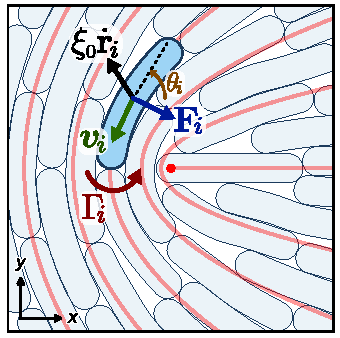
\includegraphics[width=\linewidth,page=1]{media/paper-main}
\end{minipage}
\end{wide}
\onslide<1->
\hfill{\footnotesize \colI{interactions}\quad \colA{self-propulsion \& reversals}\quad \colR{rotational noise}}
\end{frame}


\begin{frame}[t]{Extended Dean's equation}
\small\setlength{\abovedisplayskip}{3pt}\setlength{\belowdisplayskip}{3pt}
\begin{wide}{10pt}
\onslide<+->
\vspace{-2ex}
Same derivation as Dean, now over $(\r,\theta)$; exact in the white-noise limit:\par\vspace{1ex}
\begin{equation*}
    \begin{aligned}
    \partial_t\varrho_t(\r,\theta) = {}&
    \lab{\colI{\frac1{\xi_0}\pd{}{\r}\tcdot\left(\varrho_t\pd{}{\r}\frac{\delta\calF}{\delta\varrho}\right)}}{translational friction}
    + \lab{\colI{\frac1{\xir}\pd{}{\theta}\!\left(\varrho_t\pd{}{\theta}\frac{\delta\calF}{\delta\varrho}\right)}}{rotational friction}
    + \lab{\colA{\frac{v_0^2}{2\frev}\,p_\alpha(\theta)p_\beta(\theta)\,\pd{^2\varrho_t}{r_\alpha\partial r_\beta}}}{It\^o term}
    + \lab{\colR{\Lambda\,\pd{^2\varrho_t}{\theta^2}}}{rot.\ diffusion}
    \\
    &\colA{- \pd{}{\r}\tcdot\left(\sqrt{\varrho_t}\,\p(\theta)\,k(\r,\theta,t)\right)}
    \colR{- \pd{}{\theta}\!\left(\sqrt{\varrho_t}\,\lambda(\r,\theta,t)\right)}
    \qquad\text{\footnotesize noise shares $\colA{v_0^2/\frev}$ with It\^o term}
    \end{aligned}
\end{equation*}

\onslide<+->
\begin{align*}
    \colA{\la k(\r,\theta,t)\,k(\r',\theta',t')\ra} &= \frac{v_0^2}{\frev\rho_0}\;\delta(t-t')\,\delta(\r-\r')\,\delta(\theta-\theta'),
    \\
    \colR{\la \lambda(\r,\theta,t)\,\lambda(\r',\theta',t')\ra} &= \frac{2\Lambda}{\rho_0}\;\delta(t-t')\,\delta(\r-\r')\,\delta(\theta-\theta')
\end{align*}

\onslide<+->
\begin{equation*}
    \colI{\calF[\varrho]} = \frac{\rho_0^2}2\!\int\!\d\r\,\d\r'\,\d\theta\,\d\theta'\,
    V(\r\!-\!\r'\!,\theta,\theta')\,\varrho(\r,\theta)\,\varrho(\r'\!,\theta'),
    \onslide<+-> \qquad \hat\Q(\theta) = \begin{pmatrix}
        \cos 2\theta & \sin 2\theta \\
        \sin 2\theta & -\cos 2\theta
    \end{pmatrix}
\end{equation*}
Target: density $\rho(\r,t) = \int\!\d\theta\,\varrho_t(\r,\theta)$ and nematic tensor $\Q(\r,t) = \int\!\d\theta\,\varrho_t(\r,\theta)\,\hat\Q(\theta)$
\end{wide}
\end{frame}


\begin{frame}{Free energy of the nematic}
\onslide<+->
$V$ unknown $\Rightarrow$ assume $\colI{\calF}$ depends on $\varrho$ only through $\rho$ and $\Q$:
\begin{align*}
    \colI{\calF[\varrho] = F[\rho,\Q]} = \int\!\d\r\;\mathfrak f\bigl(\rho(\r),\Q(\r),\partial_\r\Q(\r)\bigr)
\end{align*}
\onslide<+->
\begin{align*}
    \mathfrak f(\rho,\Q,\partial_\r\Q) = \lab{\frac B2(\rho-1)^2}{incompressibility}
    + \lab{\frac a2(\Q\!:\!\Q) + \frac b4(\Q\!:\!\Q)^2}{Landau--de Gennes, $a<0$: order}
    + \lab{\frac K2(\partial_\r\Q)\!:\!(\partial_\r\Q)}{elasticity (one constant)}
\end{align*}
\onslide<+->
Pressure from the bulk term alone: $p = \rho\,\partial_\rho\mathfrak f_B - \mathfrak f_B$ ~~with~~ $\mathfrak f_B = \tfrac B2(\rho-1)^2$
\begin{align*}
    p = \tfrac B2\left(\rho^2-1\right) \simeq B(\rho-1)
    \qquad\text{(leading order in $\rho-1$)}
\end{align*}
\end{frame}


\begin{frame}{Density equation}
\onslide<+->
Integrate over $\theta$; leading order in $1/B$ at fixed pressure:
\begin{align*}
    \partial_t\rho = -\nabla\tcdot\Bigl[
    \frac1{\xi_0}\bigl(\lab{\colI{-B\nabla\rho}}{pressure} + \lab{\colI{\Q\!:\!\nabla\H}}{elastic} + \lab{\colA{\fa}}{active}\bigr)
    + \lab{\colA{\bEta_{\rho}(\r,t)}}{noise}\Bigr]
\end{align*}
\onslide<+->
\begin{align*}
    \colI{\H(\r)} &= -\delta F/\delta\Q = -a\Q - b(\Q\!:\!\Q)\Q + K\nabla^2\Q
    \\
    \colA{f^a_\alpha(\r)} &= -\zeta\,\partial_\beta Q_\ab(\r),
    \qquad
    \zeta = \frac{\xi_0v_0^2}{4\frev}
    \quad{\color{litegray}\Big(\leftarrow\frac{\xi_0 v_0^2}{4\frev+2\Lambda},~\Lambda\ll\frev\Big)}
    \\
    \onslide<+->{\colA{\bEta_{\rho}(\r,t)}} &\onslide<.->{= \int\!\d\theta\,\sqrt{\varrho_t(\r,\theta)}\,\p(\theta)\,k(\r,\theta,t)}
    \\
    \onslide<.->{\colA{\la \eta^{\rho}_\alpha(\r,t)\,\eta^{\rho}_\beta(\r',t') \ra}}
    &\onslide<.->{= \frac{2\zeta}{\xi_0\rho_0}\left[Q_\ab(\r)+\rho(\r)\,\delta_\ab\right]\delta(\r-\r')\,\delta(t-t')}
\end{align*}
{\footnotesize
\begin{itemize}\setlength{\itemsep}{0pt}
    \item<2-> $\colA{\fa}$: active stress $-\zeta\Q$, extensile for $\zeta>0$; largest at a defect core
    \item<3-> noise: \emph{same} $\colA{\zeta}$ as the active force; $\int\!\d\r\,\rho$ conserved per realization
\end{itemize}}
\end{frame}


\begin{frame}{Nematic field equation}
\onslide<+->
Multiply by $\hat\Q(\theta)$, integrate over $\theta$ $\Rightarrow$ not closed:
\begin{align*}
    \partial_t Q_\ab = {}& \colI{\frac1{\xi_0}\partial_i\Bigl(Q_\ab\,\partial_i\frac{\delta F}{\delta\rho}
    + \mathhlbox{liteyellow}{\langle\hat Q_\ab\hat Q_\mn\rangle_\varrho}\,\partial_i\frac{\delta F}{\delta Q_\mn}\Bigr)}
    \colI{- \frac1{\xir}\mathhlbox{liteyellow}{\langle\hat Q'_\ab\hat Q'_\mn\rangle_\varrho}\,\frac{\delta F}{\delta Q_\mn}}
    \colR{- 4\Lambda Q_\ab}
    \\
    &\colA{+ \frac{\zeta}{\xi_0}\bigl(\nabla^2Q_\ab
    + \partial_i\partial_j\mathhlbox{liteyellow}{\langle\hat Q_\ab\hat Q_{ij}\rangle_\varrho}\bigr) - \partial_i\eta^Q_{\ab i}} + \colR{f^Q_\ab}
\end{align*}

\onslide<+->
Max-entropy closure:
$\mathhlbox{liteyellow}{\langle\hat\Q\hat\Q\rangle_\varrho}\simeq\rho\J$, ~~$\mathhlbox{liteyellow}{\langle\hat\Q'\hat\Q'\rangle_\varrho}\simeq4\rho\J$

{\footnotesize lowest order, accurate to $O(S^2)$}

\vspace{-2.5cm}\hfill 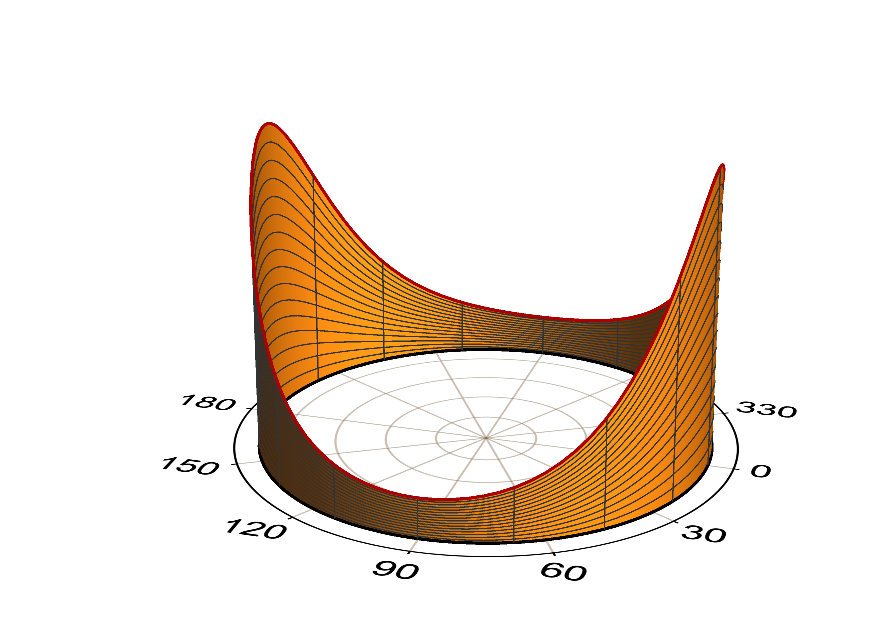
\includegraphics[width=0.3\linewidth]{media/pdf-mathematica-2}

\vspace{-1cm}
\onslide<+->
\begin{align*}
    \partial_t \Q = {}& -\nabla\!\cdot\!\Bigl[\frac1{\xi_0}
    \bigl(\colI{-\Q B \nabla\rho + \nabla \H}\bigr) + \colA{\bEta^\Q}\Bigr] + \lab{\frac4{\xir} \Ha}{relaxation} + \colR{\f^Q}
    \\
    &\Ha = -a'\Q - b(\Q\!:\!\Q)\Q + K'\nabla^2\Q,
    \\
    &a' = \colI{a}+\colR{\Lambda\xir}, \qquad K' = \colI{K}+\colA{{\zeta\xir}/({4\xi_0})}
    \qquad\text{\footnotesize renormalized by rot.\ noise and activity}
\end{align*}
\end{frame}


\begin{frame}{Fluctuating active nematic}
\onslide<+->
Closed stochastic equations for $\rho$ and $\Q$:
\begin{align*}
    \partial_t\rho ={}& -\nabla\tcdot\Bigl[
    \frac1{\xi_0}\bigl(\colI{-B\nabla\rho} + \alt<2->{{\color{litegray}\Q\!:\!\nabla\H}}{\colI{\Q\!:\!\nabla\H}} + \colA{\fa}\bigr)
    + \colA{\bEta_{\rho}(\r,t)}\Bigr]
    \\
    \partial_t \Q = {}& -\nabla\!\cdot\!\Bigl[\frac1{\xi_0}
    \bigl(\colI{-\Q B \nabla\rho} + \alt<2->{{\color{litegray}\nabla \H}}{\colI{\nabla \H}}\bigr) + \colA{\bEta^\Q}\Bigr] + \frac4{\xir} \Ha + \colR{\f^Q}
    \\[3ex]
    &\alt<2->{{\color{litegray}\H = -\delta F/\delta\Q = -a\Q - b(\Q\!:\!\Q)\Q + K\nabla^2\Q}}{\colI{\H = -\delta F/\delta\Q = -a\Q - b(\Q\!:\!\Q)\Q + K\nabla^2\Q}}
    \\
    &\Ha = -a'\Q - b(\Q\!:\!\Q)\Q + K'\nabla^2\Q,
    \qquad a' = \colI{a}+\colR{\Lambda\xir}
    \\
    &\colA{\f^a} = -\colA{\zeta}\,\nabla\cdot\Q,
    \qquad K' = \colI{K}+\colA{\zeta\xir/(4\xi_0)},
    \qquad \colA{\zeta = \frac{\xi_0v_0^2}{4\frev}}
\end{align*}
\onslide<+->
{\footnotesize
Drop the $\nabla\H$ terms:
\begin{itemize}\setlength{\itemsep}{0pt}
    \item fourth-order derivatives of $\Q$; Onsager pair $\Rightarrow$ dropped together
    \item standard in dry active nematics, also for \textit{M.\ xanthus}: $\H$ vanishes in the ordered state
\end{itemize}}
\end{frame}


\begin{frame}{Results}
\end{frame}



\begin{frame}{Summary}
    \onslide<+->
    \begin{wide}{10pt}
    \begin{minipage}[t]{0.5\linewidth}
        
        \vspace{1cm}
        \begin{itemize}
        % \setlength\itemsep{3ex}
    
        \item Microscopic model of bacterial dynamics
        \item Fluctuating active nematic equations
        \item Pressure fluctuations
        \item Nucleation theory with fluctuating barrier
    \end{itemize}

    \vspace{0.6cm}
    {\large \color{bblue} Open questions}

    \begin{itemize}
        \item Exceeding critical pressure is necessary, but not sufficient
        \item Reversal rate is not high enough to approximate the dichotomous noise by white noise
    \end{itemize}
    \end{minipage}% 
    \hfill\onslide<+->
    \begin{minipage}[t]{0.5\linewidth}
        
    {\centering
    
    \color{darkgreen} 

    \vspace{1cm}Polarity fluctuations     
    
    \vspace{0.5cm}
    $\big\downarrow$
    
    \vspace{0.5cm}
    Pressure fluctuations
    
    \vspace{0.5cm}
    $\big\downarrow$
    
    \vspace{0.5cm}
    {
    \textbf{Nucleation Theory}}
    
    \vspace{1cm}
    }
    
    \end{minipage}
    \end{wide}
    \end{frame}

\end{document}
